\documentclass[review,3p]{elsarticle}

\usepackage{lineno,hyperref}
\modulolinenumbers[5]
\usepackage{subcaption}             % used in subtable
\usepackage{amsmath,amsfonts,amsthm}            % for subequations

\usepackage{mathtools,amssymb}          % for \leqslant
\newcommand{\ddn}[2]{\frac{\mathrm{d}}{\mathrm{d}#1}#2}
\newcommand{\ddt}{\frac{\mathrm{d}}{\mathrm{d}t}}


\usepackage{upgreek}
\usepackage[dvipsnames]{xcolor}
\usepackage{soul}
\usepackage{multirow}

\usepackage{array}
\newcolumntype{C}[1]{>{\centering\let\newline\\\arraybackslash\hspace{0pt}}m{#1}} 
\newcolumntype{L}[1]{>{\raggedright\let\newline\\\arraybackslash\hspace{0pt}}m{#1}} 
\newcolumntype{R}[1]{>{\raggedleft\let\newline\\\arraybackslash\hspace{0pt}}m{#1}} 

\usepackage{booktabs}       % http://ctan.org/pkg/booktabs

\newcommand{\tabitem}{~~\llap{\textbullet}~~}           % for items inside a table
\usepackage{makecell}       % used inside a table
\usepackage{pbox}           % for weak form 3
\usepackage{empheq}
\newcommand*\widefbox[1]{\fbox{\hspace{2em}#1\hspace{2em}}}


\usepackage{colortbl}
\usepackage{esvect}
\usepackage{spreadtab}
\usepackage{numprint}
\usepackage{xstring}
\renewcommand*{\thefootnote}{\fnsymbol{footnote}}
\usepackage[symbol]{footmisc}

\usepackage{siunitx}

\makeatletter       % for rom in deal.ii symbol
\newcommand*{\rom}[1]{\expandafter\@slowromancap\romannumeral #1@}
\makeatother

\usepackage{enumitem}

\usepackage{cleveref}
\crefformat{section}{\S#2#1#3} % see manual of cleveref, section 8.2.1
\crefformat{subsection}{\S#2#1#3}
\crefformat{subsubsection}{\S#2#1#3}

\captionsetup[figure]{labelfont={bf},name={Fig.},labelsep=period}
\captionsetup[table]{labelfont={bf},name={Table},labelsep=space}

\usepackage[labelformat=simple]{subcaption}	        	% order of subfigure with brackets
\renewcommand\thesubfigure{(\alph{subfigure})}
\renewcommand\thesubtable{(\alph{subtable})}


\usepackage{graphicx}
\usepackage{wrapfig}
\usepackage{lipsum}

\usepackage{pgfplots}       % for tikzpicture

\pdfsuppresswarningpagegroup=1      % eliminate warning 'multiple pdfs with page group included in a single page'

\usepackage[ruled,linesnumbered]{algorithm2e}		% for algorithm


\begin{document}

\section{Influence of $d(x)$ and $r(x)$ on \texorpdfstring{$\alpha_{\rm R}$}{alpha_{rm R}}}         \label{discretization_error_bench_pois_diff_Helm}

If not stated otherwise, $P_2$ elements are used for the standard FEM, and $P_4/P_3^{\rm disc}$ elements are used for the mixed FEM.

%\subsection{\texorpdfstring{$p=(2\pi c_1)^{-2}\sin(2\pi c_1x)$}{p=(2pic1){-2}sin(2pic1x)}}
%
%\subsubsection{d=10, r=0}
%
%
%\begin{table}[!ht]
%\caption[sss]{Ratio of $\alpha_{\rm R}$ for $d=10$ to that for $d=1$.}
%\label{evolution_convergence_order_sample_equations}
%\centering
% \begin{tabular}{c c c c c c c} \hline
% \multirow{2}{*}{$c$} & \multicolumn{3}{c}{The standard FEM} & \multicolumn{3}{c}{The mixed FEM} \\ \cline{2-4} \cline{5-7}
% & $u$ & $u_x$ & $u_{xx}$ & $u$ & $u_x$ & $u_{xx}$ \\	\hline
%$10^{-2}$ & 0.8 & 1.0 & 1.0 & 1.0 & 10.0 & 10.0 \\ 
%$10^{-1}$ & 0.8 & 1.0 & 1.0 & 1.0 & 10.0 & 10.0 \\ 
%$10^{0}$ & 1.0 & 0.5 & 1.0 & 0.1 & 10.0 & 10.0 \\ 
%$10^{1}$ & 1.3 & 0.5 & 1.0 & 1.0 & 10.0 & 10.0 \\ 
%$10^{2}$ & 1.3 & 1.3 & 1.0 & 1.0 & 10.0 & 10.0 \\ \hline
%\end{tabular}
%\end{table}
% \newpage

\subsection{\texorpdfstring{p=$e^{-(x-0.5)^2}$}{p=e^{-(x-0.5)^2}}}			\label{p_exp_2_diff_2_Helm}

\subsubsection{d=1+0.5\texorpdfstring{$\sin$(cx)}{sin(cx)}, r=0}            \label{p_exp_d_1plus0p5sin_r_0}

For $c$ being 1, 10 and 100, shapes of $d$ are shown in Fig.~\ref{shape_1_plus_sincx}, and $\|d\|_2$ are 1.23, 1.14 and 1.06, respectively. 
The analytical order of convergence can be reached within a number of $h$-refinements, and $\alpha_{\rm R}$ are shown in Fig.~\ref{alpha_R_benchmark_Pois2diff2Helm}, which are independent of $d$.

 \begin{figure}[!ht]
 \centering
     \includegraphics[width=0.5\linewidth]{py_var_1_plus_sincx.pdf}
     \caption{Shape of $d=1+0.5\sin(cx)$ for $c$ being 1, 10, 100.}
     \label{shape_1_plus_sincx}
 \end{figure}

\begin{figure}[!ht]
\hspace{0.0cm}
\begin{subfigure}[b]{0.35\textwidth}
\scalebox{0.85}{
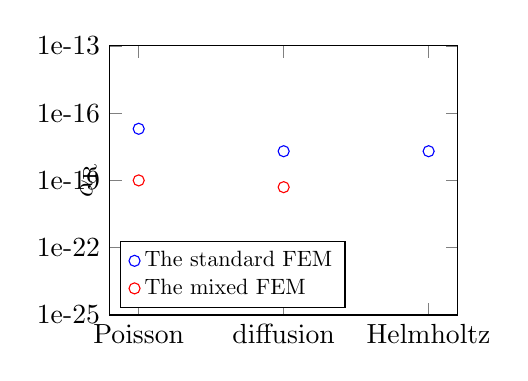
\begin{tikzpicture} 
\begin{axis}
[
    ymode=log,    
    ymin=1e-25,
    ymax=1e-13,
    ytick={1e-25, 1e-22, 1e-19, 1e-16, 1e-13},
    yticklabels={1e-25, 1e-22, 1e-19, 1e-16, 1e-13},      
    legend style={nodes={scale=0.8},at={(0.03,0.15)},anchor=west},
    legend cell align={left},
    height=5cm,
    width=6cm,
    ylabel={$\alpha_{\rm R}$},
    ylabel style={at={(-0.01,0.5)}},    
    xtick={0,1,2,3,4},
    xticklabels={Poisson, diffusion, Helmholtz}
]
\addplot[blue,mark=o, only marks,mark options={color=blue,fill=blue}] coordinates {(0,2.0e-17) (1,2.0e-18) (2,2.0e-18)};	% SM

\addplot[red,mark=o, only marks,mark options={color=red,fill=red}] coordinates {(0,1.0e-19) (1,5.0e-20) (2,1.0e-30)};		% MM

%\addplot[blue,mark=o, only marks,mark options={color=blue!80,fill=blue}] coordinates {(0,2.0e-30) (1,2.0e-30) (2,2.0e-18)};	% SM_supp_Helm
%\addplot[blue,mark=o, only marks,mark options={color=blue!60,fill=blue}] coordinates {(0,2.0e-30) (1,2.0e-30) (2,2.0e-20)};

%\addplot[blue,mark=o, only marks,mark options={color=blue!40,fill=blue}] coordinates {(0,2.0e-30) (1,2.0e-30) (2,2.0e-22)};
%\addplot[blue,mark=o, only marks,mark options={color=blue!20,fill=blue}] coordinates {(0,2.0e-30) (1,2.0e-30) (2,2.0e-24)};

\legend{The standard FEM, The mixed FEM};
\end{axis}
\end{tikzpicture}
}
\vspace{-0.7cm}
\caption{Solution}
\label{alpha_R_Poisson_benchmark_2_diff_2_Helm_solu}
\end{subfigure}
\hspace{-0.7cm}
\begin{subfigure}[b]{0.35\textwidth}
\scalebox{0.85}{
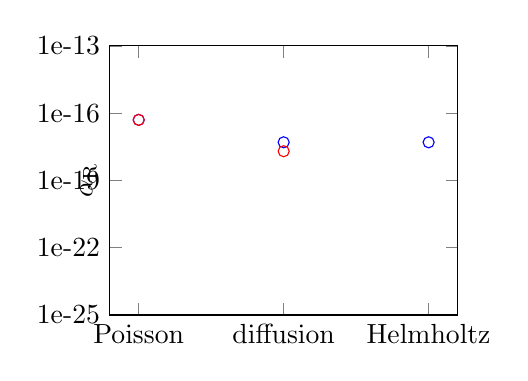
\begin{tikzpicture} 
\begin{axis}
[
    ymode=log,    
    ymin=1e-25,
    ymax=1e-13,
    ytick={1e-25, 1e-22, 1e-19, 1e-16, 1e-13},
    yticklabels={1e-25, 1e-22, 1e-19, 1e-16, 1e-13},   
    legend style={nodes={scale=0.8},at={(0.03,0.85)},anchor=west},
    legend cell align={left},
    height=5cm,
    width=6cm,
    ylabel={$\alpha_{\rm R}$},
    ylabel style={at={(-0.01,0.5)}},    
    xtick={0,1,2,3,4},
    xticklabels={Poisson, diffusion, Helmholtz}
]
\addplot[blue,mark=o, only marks,mark options={color=blue,fill=blue}] coordinates {(0,5.0e-17) (1,5.0e-18) (2,5.0e-18)};
\addplot[red,mark=o, only marks,mark options={color=red,fill=red}] coordinates {(0,5.0e-17) (1,2.0e-18) (2,1.0e-30)};

%\addplot[blue,mark=o, only marks,mark options={color=blue!80,fill=blue}] coordinates {(0,2.0e-30) (1,2.0e-30) (2,5.0e-18)};
%\addplot[blue,mark=o, only marks,mark options={color=blue!60,fill=blue}] coordinates {(0,2.0e-30) (1,2.0e-30) (2,1.0e-19)};
%\addplot[blue,mark=o, only marks,mark options={color=blue!40,fill=blue}] coordinates {(0,2.0e-30) (1,2.0e-30) (2,1.0e-20)};
%\addplot[blue,mark=o, only marks,mark options={color=blue!20,fill=blue}] coordinates {(0,2.0e-30) (1,2.0e-30) (2,5.0e-21)};
\end{axis}
\end{tikzpicture}
}
\vspace{-0.7cm}
\caption{First derivative}
\label{alpha_R_Poisson_benchmark_2_diff_2_Helm_grad}
\end{subfigure}
\hspace{-0.7cm}
\begin{subfigure}[b]{0.35\textwidth}
\scalebox{0.85}{
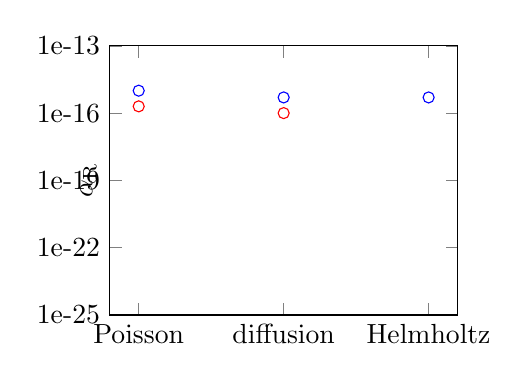
\begin{tikzpicture} 
\begin{axis}
[
    ymode=log,    
    ymin=1e-25,
    ymax=1e-13,
    ytick={1e-25, 1e-22, 1e-19, 1e-16, 1e-13},
    yticklabels={1e-25, 1e-22, 1e-19, 1e-16, 1e-13},     
    legend style={nodes={scale=0.8},at={(0.03,0.85)},anchor=west},
    legend cell align={left},
    height=5cm,
    width=6cm,
    ylabel={$\alpha_{\rm R}$},
    ylabel style={at={(-0.01,0.5)}},    
    xtick={0,1,2,3,4},
    xticklabels={Poisson, diffusion, Helmholtz} 
]
\addplot[blue,mark=o, only marks,mark options={color=blue,fill=blue}] coordinates {(0,1.0e-15) (1,5.0e-16) (2,5.0e-16)};	% SM

\addplot[red,mark=o, only marks,mark options={color=red,fill=red}] coordinates {(0,2.0e-16) (1,1.0e-16) (2,2.0e-30)};		% MM

%\addplot[blue,mark=o, only marks,mark options={color=blue!80,fill=blue}] coordinates {(0,2.0e-30) (1,2.0e-30) (2,2.0e-30)};	% SM_supp_diff
%\addplot[blue,mark=o, only marks,mark options={color=blue!60,fill=blue}] coordinates {(0,2.0e-30) (1,2.0e-30) (2,2.0e-30)};
%\addplot[blue,mark=o, only marks,mark options={color=blue!40,fill=blue}] coordinates {(0,2.0e-30) (1,2.0e-30) (2,2.0e-30)};
%\addplot[blue,mark=o, only marks,mark options={color=blue!20,fill=blue}] coordinates {(0,2.0e-30) (1,2.0e-30) (2,2.0e-30)};

\end{axis}
\end{tikzpicture}
}
\vspace{-0.7cm}
\caption{Second derivative}
\label{alpha_R_Poisson_benchmark_2_diff_2_Helm_2ndd}
\end{subfigure}
\caption{Influence of $d(x)$ and $r(x)$ on $\alpha_{\rm R}$ for $p=e^{-(x-0.5)^2}$.}
\label{alpha_R_benchmark_Pois2diff2Helm}
\end{figure}

%for the Poisson, diffusion and Hemlholtz equations for section \ref{p_exp_2_diff_2_Helm}

%\newpage



%\paragraph{The standard FEM}
%
%When $c$ is smaller than or equal to 10, both the truncation error and round-off error are not affected by $c$.	
%When $c$ is larger than 10, the truncation error becomes larger, and $\alpha_{\rm R}$ increases.
%
%\paragraph{The mixed FEM}
%
%The truncation error tends to increase when $c$ increases, but $\alpha_{\rm R}$ are not affected.

% \newpage

\subsubsection{d=1+0.5\texorpdfstring{$\sin$(x)}{sin(x)}, r=c}

Here, $c$ is chosen to be 1, 10 and 100. 
It is found that both the truncation error $E_{\rm T}$ and round-off error $E_{\rm R}$ are independent of $c$.


%$\alpha_{\rm R}$ for different $c$ are summarized in Fig.~\ref{alpha_R_benchmark_Pois2diff2Helm}.
%For larger $c$, $\alpha_{\rm R}$ is denoted by lighter colors.
%Last but not least, the offsets $\alpha_{\rm R}$ for the diffusion equation tend to be smaller than that for the Poisson equation.

\newpage
\subsection{\texorpdfstring{p=$\sin$(2$\pi$x)}{p=sin(2pix)}} \label{discretization_error_bench_diff}

\begin{figure}[!ht]
\hspace{0.0cm}
\begin{subfigure}[b]{0.35\textwidth}
\scalebox{0.85}{
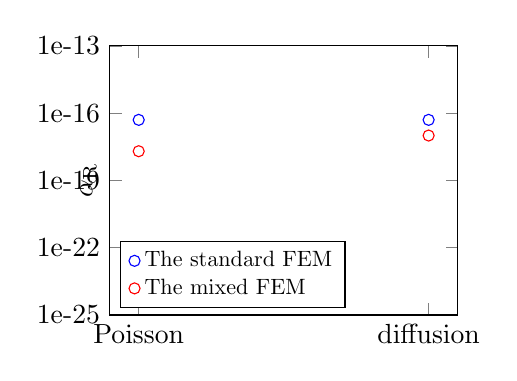
\begin{tikzpicture} 
\begin{axis}
[
    ymode=log,    
    ymin=1e-25,
    ymax=1e-13,
    ytick={1e-25, 1e-22, 1e-19, 1e-16, 1e-13},
    yticklabels={1e-25, 1e-22, 1e-19, 1e-16, 1e-13},      
    legend style={nodes={scale=0.8},at={(0.03,0.15)},anchor=west},
    legend cell align={left},
    height=5cm,
    width=6cm,
    ylabel={$\alpha_{\rm R}$},
    ylabel style={at={(-0.01,0.5)}},    
    xtick={0,1,2,3,4},
    xticklabels={Poisson, diffusion, Helmholtz}
]
\addplot[blue,mark=o, only marks,mark options={color=blue,fill=blue}] coordinates {(0,5.0e-17) (1,5.0e-17) (2,5.0e-30)};	%

\addplot[red,mark=o, only marks,mark options={color=red,fill=red}] coordinates {(0,2.0e-18) (1,1.0e-17) (2,5.0e-30)};		%

\addplot[blue,mark=o, only marks,mark options={color=blue!80,fill=blue}] coordinates {(0,2.0e-30) (1,2.0e-30) (2,2.0e-30)};	%
\addplot[blue,mark=o, only marks,mark options={color=blue!60,fill=blue}] coordinates {(0,2.0e-30) (1,2.0e-30) (2,2.0e-30)};
\addplot[blue,mark=o, only marks,mark options={color=blue!40,fill=blue}] coordinates {(0,2.0e-30) (1,2.0e-30) (2,2.0e-30)};
\addplot[blue,mark=o, only marks,mark options={color=blue!20,fill=blue}] coordinates {(0,2.0e-30) (1,2.0e-30) (2,2.0e-30)};
\legend{The standard FEM, The mixed FEM};
\end{axis}
\end{tikzpicture}
}
\vspace{-0.2cm}
\caption{Solution}
\label{alpha_R_Poisson_p_sin2pix}
\end{subfigure}
\hspace{-0.7cm}
\begin{subfigure}[b]{0.35\textwidth}
\scalebox{0.85}{
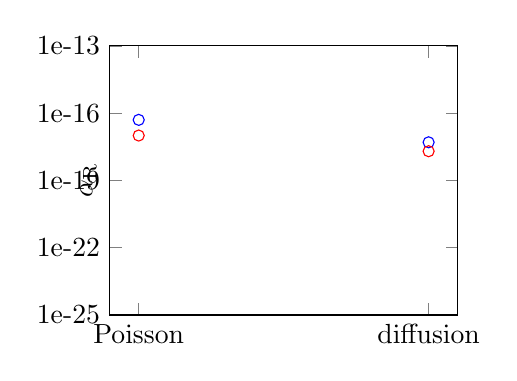
\begin{tikzpicture} 
\begin{axis}
[
    ymode=log,    
    ymin=1e-25,
    ymax=1e-13,
    ytick={1e-25, 1e-22, 1e-19, 1e-16, 1e-13},
    yticklabels={1e-25, 1e-22, 1e-19, 1e-16, 1e-13},   
    legend style={nodes={scale=0.8},at={(0.03,0.85)},anchor=west},
    legend cell align={left},
    height=5cm,
    width=6cm,
    ylabel={$\alpha_{\rm R}$},
    ylabel style={at={(-0.01,0.5)}},    
    xtick={0,1,2,3,4},
    xticklabels={Poisson, diffusion, Helmholtz}
]
\addplot[blue,mark=o, only marks,mark options={color=blue,fill=blue}] coordinates {(0,5.0e-17) (1,5.0e-18) (2,5.0e-30)};
\addplot[red,mark=o, only marks,mark options={color=red,fill=red}] coordinates {(0,1.0e-17) (1,2.0e-18) (2,1.0e-30)};
\addplot[blue,mark=o, only marks,mark options={color=blue!80,fill=blue}] coordinates {(0,2.0e-30) (1,2.0e-30) (2,5.0e-30)};
\addplot[blue,mark=o, only marks,mark options={color=blue!60,fill=blue}] coordinates {(0,2.0e-30) (1,2.0e-30) (2,1.0e-30)};
\addplot[blue,mark=o, only marks,mark options={color=blue!40,fill=blue}] coordinates {(0,2.0e-30) (1,2.0e-30) (2,1.0e-30)};
\addplot[blue,mark=o, only marks,mark options={color=blue!20,fill=blue}] coordinates {(0,2.0e-30) (1,2.0e-30) (2,5.0e-30)};
\end{axis}
\end{tikzpicture}
}
\vspace{-0.2cm}
\caption{First derivative}
\label{alpha_R_Poisson_p_sin2pix_2_diffusion}
\end{subfigure}
\hspace{-0.7cm}
\begin{subfigure}[b]{0.35\textwidth}
\scalebox{0.85}{
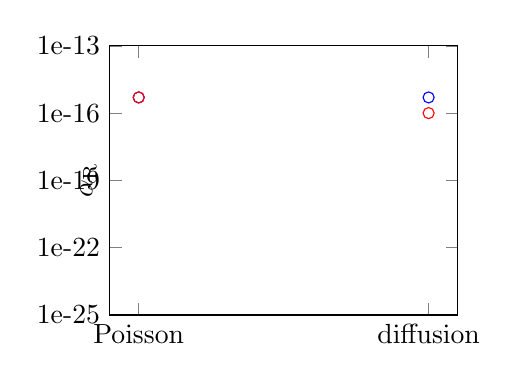
\begin{tikzpicture} 
\begin{axis}
[
    ymode=log,    
    ymin=1e-25,
    ymax=1e-13,
    ytick={1e-25, 1e-22, 1e-19, 1e-16, 1e-13},
    yticklabels={1e-25, 1e-22, 1e-19, 1e-16, 1e-13},     
    legend style={nodes={scale=0.8},at={(0.03,0.85)},anchor=west},
    legend cell align={left},
    height=5cm,
    width=6cm,
    ylabel={$\alpha_{\rm R}$},
    ylabel style={at={(-0.01,0.5)}},    
    xtick={0,1,2,3,4},
    xticklabels={Poisson, diffusion, Helmholtz} 
]
\addplot[blue,mark=o, only marks,mark options={color=blue,fill=blue}] coordinates {(0,5.0e-16) (1,5.0e-16) (2,5.0e-30)};
\addplot[red,mark=o, only marks,mark options={color=red,fill=red}] coordinates {(0,5.0e-16) (1,1.0e-16) (2,2.0e-30)};
\end{axis}
\end{tikzpicture}
}
\vspace{-0.2cm}
\caption{Second derivative}
\label{alpha_R_Poisson_p_sin2pix_2_Helmholtz}
\end{subfigure}
\caption{$\alpha_{\rm R}$ for the Poisson, diffusion and Hemlholtz equations with $p=\sin(2\pi x)$.}
\label{alpha_R_Poisson_p_sin2pix_2diff2helm}
\end{figure}

\subsubsection{d=1+cx}

$c$ ranges from $10^{-4}$ to $10^4$. The values of $\|d\|_2$ for different $c$ are given in Fig.~\ref{Fig:d_L2_varying_with_c_diff}.
It shows that when $c<1$, $\|d\|_2$ are basically the same; when $c>1$, $\|d\|_2$ increases quickly.

\begin{figure}[!ht]
\centering
    \includegraphics[width=0.45\linewidth]{d_L2_varying_with_c_diff.png}
    \caption{Change of $\|d\|_2$ with the coefficient $c$ for the diffusion equation.}
    \label{Fig:d_L2_varying_with_c_diff}   
\end{figure}

% \newpage
\paragraph{The standard FEM}

Using scheme $S$, the errors are shown in Fig.~\ref{py_oned_bench_diff_SM_error_scheme_S_coeff_variant}.
When $c<1$, like $\|d\|_2$, $\alpha_{\rm R}$ for different $c$ are basically the same; when $c>1$, $\alpha_{\rm R}$ increases with $c$, and the magnitude of the increase is larger for higher-order derivatives.

\begin{figure}[!ht]
    \begin{subfigure}{5.5cm}
        \includegraphics[width=1.0\linewidth]{py_oned_bench_diff_SM_error_scheme_S_coeff_variant_solu.pdf}
        \caption{Solution}
        \label{py_oned_bench_diff_SM_error_scheme_S_coeff_variant_solu}
    \end{subfigure}
    \hspace{-0.2cm}
    \begin{subfigure}{5.5cm}
        \includegraphics[width=1.0\linewidth]{py_oned_bench_diff_SM_error_scheme_S_coeff_variant_grad.pdf}
        \caption{First derivative}
        \label{py_oned_bench_diff_SM_error_scheme_S_coeff_variant_grad}
    \end{subfigure}
    \hspace{-0.2cm}
    \begin{subfigure}{5.5cm}
        \includegraphics[width=1.0\linewidth]{py_oned_bench_diff_SM_error_scheme_S_coeff_variant_2ndd.pdf}
        \caption{Second derivative}
        \label{py_oned_bench_diff_SM_error_scheme_S_coeff_variant_2ndd}
    \end{subfigure}
\caption{Absolute errors for the benchmark diffusion equation using the standard FEM with scheme $S$, $c$ variant.}
\label{py_oned_bench_diff_SM_error_scheme_S_coeff_variant}
\end{figure}


\begin{figure}[!ht]
    \begin{subfigure}{5.5cm}
        \includegraphics[width=1.0\linewidth]{py_error_oned_diff_p_sin2pix_d_1pcx_S1_degree_var_solu.pdf}
        \caption{Solution}
        \label{py_error_oned_diff_p_sin2pix_d_1pcx_S1_degree_var_solu}
    \end{subfigure}
    \hspace{-0.2cm}
    \begin{subfigure}{5.5cm}
        \includegraphics[width=1.0\linewidth]{py_error_oned_diff_p_sin2pix_d_1pcx_S1_degree_var_grad.pdf}
        \caption{First derivative}
        \label{py_error_oned_diff_p_sin2pix_d_1pcx_S1_degree_var_grad}
    \end{subfigure}
    \hspace{-0.2cm}
    \begin{subfigure}{5.5cm}
        \includegraphics[width=1.0\linewidth]{py_error_oned_diff_p_sin2pix_d_1pcx_S1_degree_var_2ndd.pdf}
        \caption{Second derivative}
        \label{py_error_oned_diff_p_sin2pix_d_1pcx_S1_degree_var_2ndd}
    \end{subfigure}
\caption{Absolute errors for the benchmark diffusion equation using the standard FEM with scheme $S$, $c$=1e4, degree variant.}
\label{py_error_oned_diff_p_sin2pix_d_1pcx_S1_degree_var}
\end{figure}




\begin{figure}[!ht]
    \begin{subfigure}{5.5cm}
        \includegraphics[width=1.0\linewidth]{py_error_oned_diff_p_sin2pix_d_1pcx_S1_c_var_solu.pdf}
        \caption{Solution}
        \label{py_error_oned_diff_p_sin2pix_d_1pcx_S1_c_var_solu}
    \end{subfigure}
    \hspace{-0.2cm}
    \begin{subfigure}{5.5cm}
        \includegraphics[width=1.0\linewidth]{py_error_oned_diff_p_sin2pix_d_1pcx_S1_c_var_grad.pdf}
        \caption{First derivative}
        \label{py_error_oned_diff_p_sin2pix_d_1pcx_S1_c_var_grad}
    \end{subfigure}
    \hspace{-0.2cm}
    \begin{subfigure}{5.5cm}
        \includegraphics[width=1.0\linewidth]{py_error_oned_diff_p_sin2pix_d_1pcx_S1_c_var_2ndd.pdf}
        \caption{Second derivative}
        \label{py_error_oned_diff_p_sin2pix_d_1pcx_S1_c_var_2ndd}
    \end{subfigure}
\caption{Absolute errors for the benchmark diffusion equation but only imposed by Dirichlet boundary conditions using the standard FEM with scheme $S$, $c$ variant.}
\label{py_error_oned_diff_p_sin2pix_d_1pcx_S1_c_var}
\end{figure}

Fig.~\ref{py_error_oned_diff_p_sin2pix_d_1pcx_S1_degree_var} proves that the element degree does not affect the round-off error.
Fig.~\ref{py_error_oned_diff_p_sin2pix_d_1pcx_S1_c_var} proves that only using Dirichlet boundary conditions produces smaller $\alpha_{\rm R}$.

% \newpage
\paragraph{The mixed FEM}
Not using scaling, the errors are shown in Fig.~\ref{py_oned_bench_diff_M0_error_coeff_variant_nonpost}.
It shows that when $c$ is relatively large, $\alpha_{\rm R}$ for the first and second derivatives increases. This is because the magnitude of the first derivative, which is $\|du_x\|_2$, increases with $c$ when $c>1$.

\begin{figure}[!ht]
    \begin{subfigure}{5.5cm}
        \includegraphics[width=1.0\linewidth]{py_oned_bench_diff_M0_error_coeff_variant_nonpost_solu.pdf}
        \caption{Solution}
        \label{py_oned_bench_diff_M0_error_coeff_variant_nonpost_solu}
    \end{subfigure}
    \hspace{-0.2cm}
    \begin{subfigure}{5.5cm}
        \includegraphics[width=1.0\linewidth]{py_oned_bench_diff_M0_error_coeff_variant_nonpost_grad.pdf}
        \caption{First derivative}
        \label{py_oned_bench_diff_M0_error_coeff_variant_nonpost_grad}
    \end{subfigure}
    \hspace{-0.2cm}
    \begin{subfigure}{5.5cm}
        \includegraphics[width=1.0\linewidth]{py_oned_bench_diff_M0_error_coeff_variant_nonpost_2ndd.pdf}
        \caption{Second derivative}
        \label{py_oned_bench_diff_M0_error_coeff_variant_nonpost_2ndd}
    \end{subfigure}
\caption{Absolute errors for the benchmark diffusion equation using the mixed FEM with $P_4/P_3^{\rm disc}$ elements, $v=-du_x$, coefficient variant, no scaling.}
\label{py_oned_bench_diff_M0_error_coeff_variant_nonpost}
\end{figure}

% \newpage

If we use scheme $M_1$ in \cite{liu2019balancing}, the errors are shown in Fig.~\ref{py_oned_bench_diff_M1_error_coeff_variant_nonpost}, where the convergence behavior of $\alpha_{\rm R}$ is observed. Note that, $\|v\|_2$ is $\|du_x\|_2$ for the diffusion equation.

\begin{figure}[!ht]
    \begin{subfigure}{5.5cm}
        \includegraphics[width=1.0\linewidth]{py_oned_bench_diff_M1_error_coeff_variant_nonpost_solu.pdf}
        \caption{Solution}
        \label{py_oned_bench_diff_M1_error_coeff_variant_nonpost_solu}
    \end{subfigure}
    \hspace{-0.2cm}
    \begin{subfigure}{5.5cm}
        \includegraphics[width=1.0\linewidth]{py_oned_bench_diff_M1_error_coeff_variant_nonpost_grad.pdf}
        \caption{First derivative}
        \label{py_oned_bench_diff_M1_error_coeff_variant_nonpost_grad}
    \end{subfigure}
    \hspace{-0.2cm}
    \begin{subfigure}{5.5cm}
        \includegraphics[width=1.0\linewidth]{py_oned_bench_diff_M1_error_coeff_variant_nonpost_2ndd.pdf}
        \caption{Second derivative}
        \label{py_oned_bench_diff_M1_error_coeff_variant_nonpost_2ndd}
    \end{subfigure}
\caption{Absolute errors for the benchmark diffusion equation using the mixed FEM with $P_4/P_3^{\rm disc}$ elements, $v=-du_x$, coefficient variant, scheme $M_1$.}
\label{py_oned_bench_diff_M1_error_coeff_variant_nonpost}
\end{figure}



\bibliographystyle{unsrt}  
\bibliography{mybibfile}  %%% Remove comment to use the external .bib file (using bibtex).


\end{document}
